\subsection{Sequence Diagram}

\begin{figure}[H]
    \centering
    \fbox{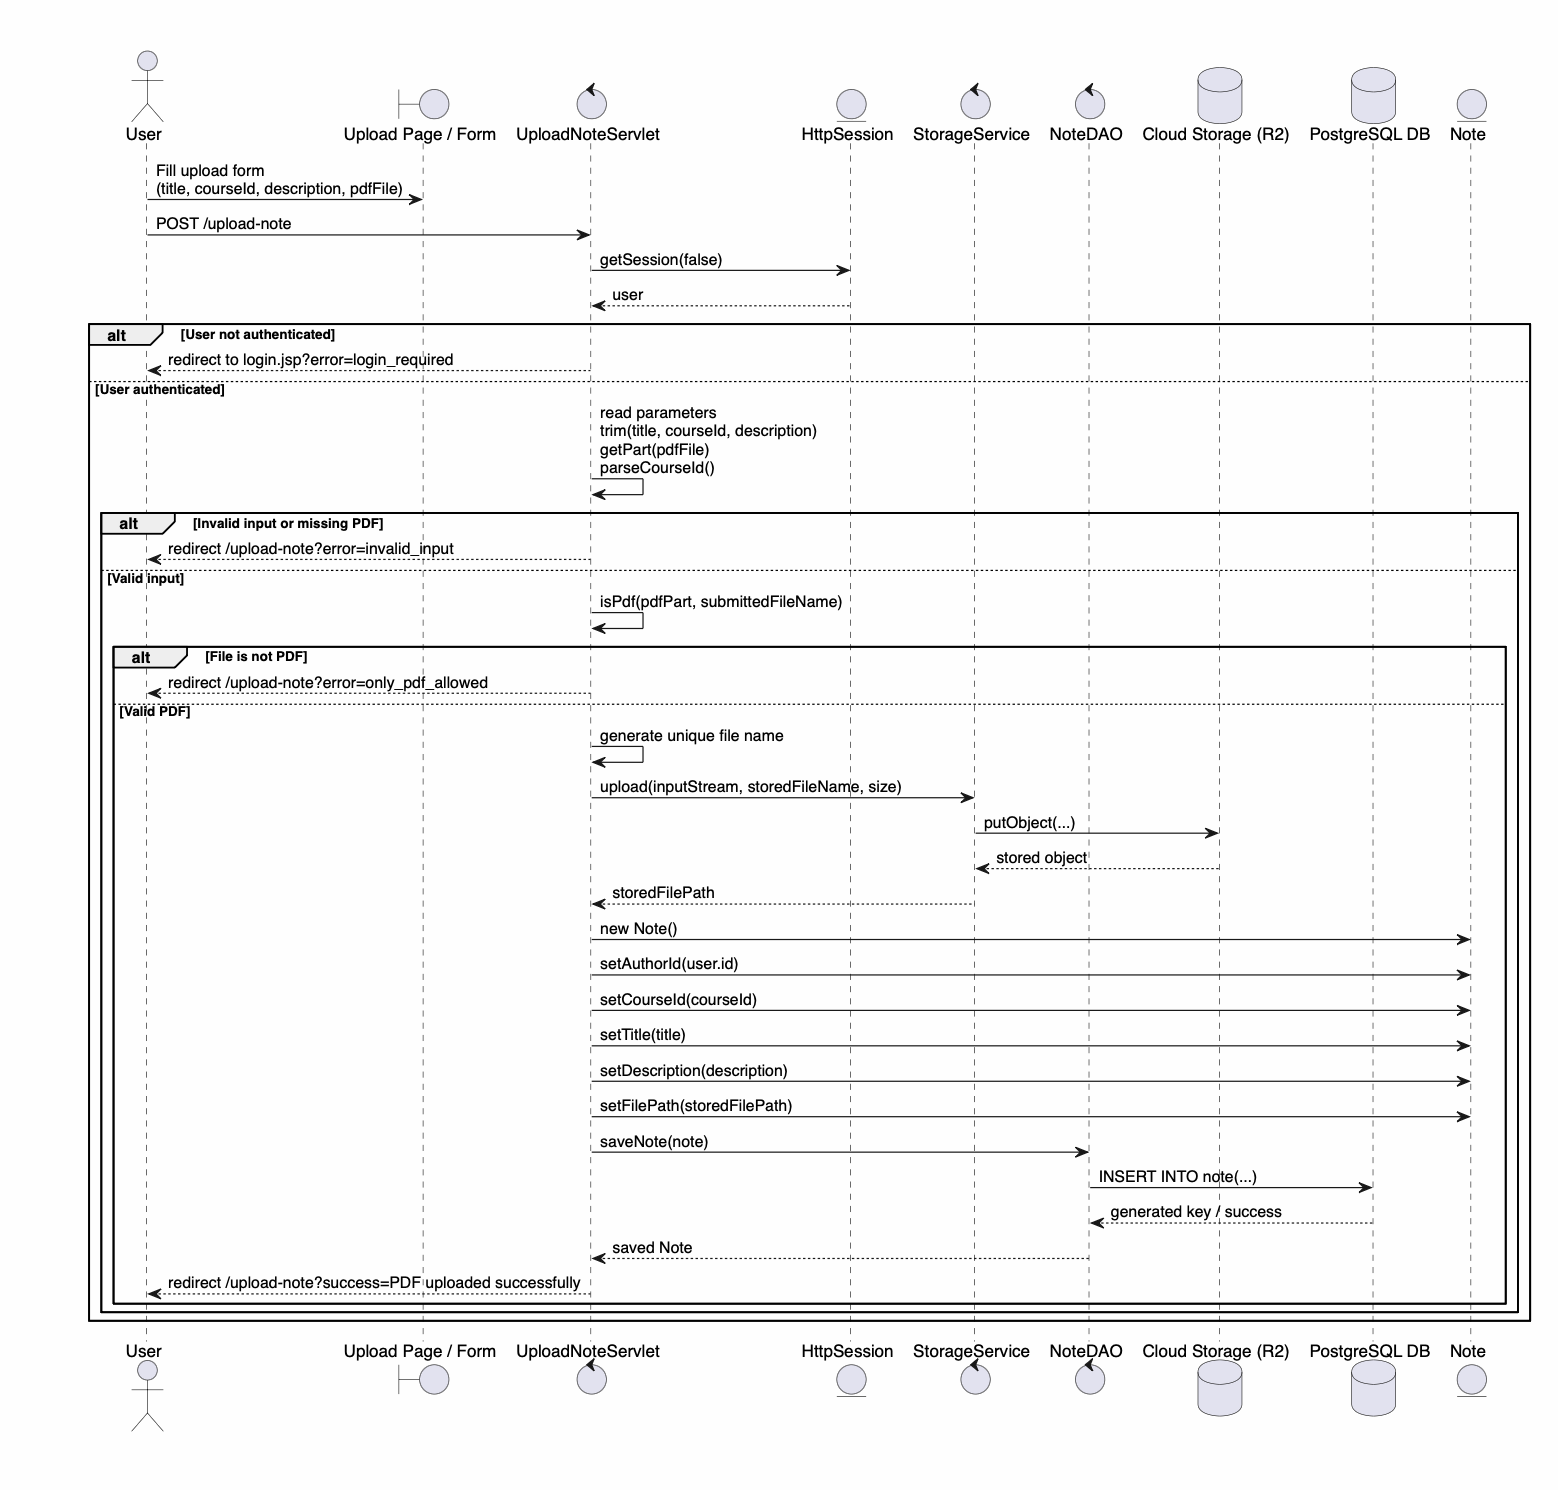
\includegraphics[width=\textwidth]{diagrams/sequenceDiagram.png}}
    \caption{Sequence Diagram -- Note Upload Flow}
    \label{fig:sequence-diagram}
\end{figure}

A representative interaction of the system is illustrated through the note upload process,
which is one of the core functionalities of the application.

The sequence diagram in Figure~\ref{fig:sequence-diagram} shows how the different components
collaborate during this operation.

When the user submits the upload form, a \texttt{POST multipart/form-data} request is sent
to the \texttt{/upload-note} endpoint. The \texttt{UploadNoteServlet} handles the request by
first verifying the existence of a valid user session. If the user is not authenticated,
the request is rejected and the user is redirected to the login page.

If the session is valid, the servlet extracts and validates the input parameters, including
the note metadata and the uploaded file. The system ensures that all required fields are
provided and that the file is in PDF format.

Once validated, a unique file name is generated and the file is uploaded to cloud storage
through the \texttt{StorageService}. The service interacts with the storage backend to persist the file and returns the file path.

Subsequently, the servlet creates a \texttt{Note} object containing all relevant metadata,
such as author, course, title, description, and file path. This object is then passed to
\texttt{NoteDAO}, which stores the information in the PostgreSQL database.

Finally, depending on the outcome of the operation, the user is redirected either to a
success page or to an error page.

This sequence diagram effectively highlights the interaction between presentation,
business logic, and data layers, providing a clear view of the system workflow.
